%!TEX root = ../template.tex
%%%%%%%%%%%%%%%%%%%%%%%%%%%%%%%%%%%%%%%%%%%%%%%%%%%%%%%%%%%%%%%%%%%%
%% chapter7.tex
%% NOVA thesis document file
%%
%% Chapter with lots of dummy text
%%%%%%%%%%%%%%%%%%%%%%%%%%%%%%%%%%%%%%%%%%%%%%%%%%%%%%%%%%%%%%%%%%%%

\typeout{NT FILE chapter7.tex}%

\chapter{Red-Black Ant Colony System}
\label{chapt:6}

\section{Introduzione}

Questo capitolo presenta una versione modificata dell'algoritmo \Gls{ACS}, chiamata Red-Black Ant Colony System (\Gls{RB-ACS}), che mira a migliorare le prestazioni dell'\Gls{ACS} su istanze di grandi dimensioni del \Gls{TSP}. Il \Gls{RB-ACS} incorpora diverse migliorie chiave all'approccio  \Gls{ACS} standard, tra cui la ricerca in parallelo, l'inizializzazione migliorata dei feromoni e l'impostazione di parametri differenziati per i due gruppi di formiche. Queste modifiche sono progettate per consentire al \Gls{RB-ACS} di esplorare lo spazio di ricerca in modo più efficace e di convergere efficientemente verso soluzioni ottimali o quasi-ottimali, anche per problemi di \Gls{TSP} su larga scala \cite{Hassan2013}.

\section{L'Algoritmo Red-Black Ant Colony System (\Gls{RB-ACS})}
Mentre l'algoritmo  \Gls{ACS} standard si è dimostrato efficace nella risoluzione di istanze del \Gls{TSP}, le sue prestazioni possono peggiorare all'aumentare delle dimensioni del problema. Il Red-Black Ant Colony System (\Gls{RB-ACS})  introduce diverse modifiche chiave all'approccio  \Gls{ACS} standard per migliorarne la scalabilità e la qualità delle soluzioni per problemi di \Gls{TSP} su larga scala \cite{Hassan2013}.

\begin{figure}[h!]
	\centering
	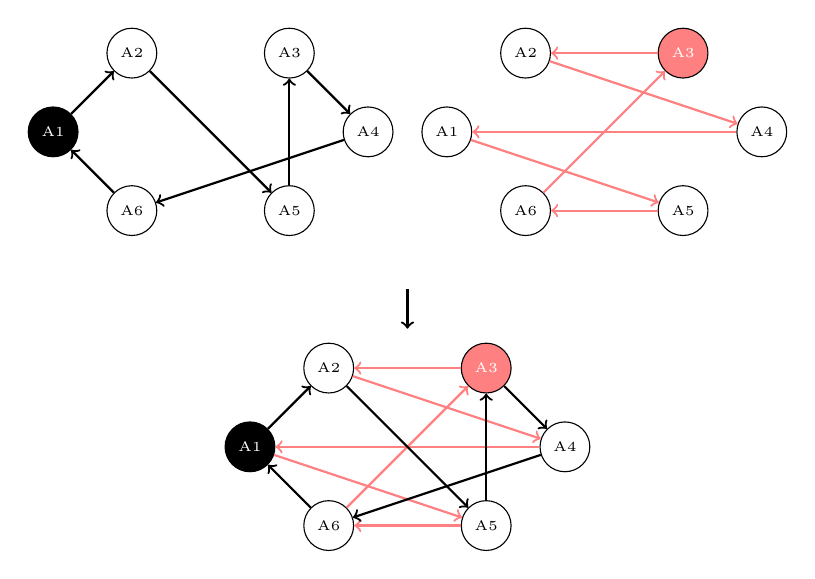
\begin{tikzpicture}[node distance=1.5cm]
		% Left diagram
		\node[circle,draw, fill=black, text=white] (A1) at (-2,0) {\tiny A1};
		\node[circle,draw] (A2) at (-1,1) {\tiny A2};
		\node[circle,draw] (A3) at (1,1) {\tiny A3};
		\node[circle,draw] (A4) at (2,0) {\tiny A4};
		\node[circle,draw] (A5) at (1,-1) {\tiny A5};
		\node[circle, draw] (A6) at (-1, -1) {\tiny A6};

		\draw[->,thick] (A1) -- (A2);
		\draw[->,thick] (A2) -- (A5);
		\draw[->,thick] (A5) -- (A3);
		\draw[->,thick] (A3) -- (A4);
		\draw[->, thick] (A6) -- (A1);
		\draw[->, thick] (A4) -- (A6);

		% Right diagram

		\node[circle,draw] (A1) at (-2 + 5,0) {\tiny A1};
		\node[circle,draw] (A2) at (-1 + 5,1) {\tiny A2};
		\node[circle,draw, fill=red!50, text = white] (A3) at (1+5,1) {\tiny A3};
		\node[circle,draw] (A4) at (2+5,0) {\tiny A4};
		\node[circle,draw] (A5) at (1+5,-1) {\tiny A5};
		\node[circle, draw] (A6) at (-1+5, -1) {\tiny A6};

		\draw[->,thick, color = red!50] (A3) -- (A2);
		\draw[->,thick, color = red!50] (A2) -- (A4);
		\draw[->,thick, color = red!50] (A4) -- (A1);
		\draw[->,thick, color = red!50] (A1) -- (A5);
		\draw[->, thick, color = red!50] (A5) -- (A6);
		\draw[->, thick, color = red!50] (A6) -- (A3);


		% Connecting arrow
		\draw[->, thick] (2.5,-2) -- (2.5,-2.5);

		\node[circle,draw, fill=black, text=white] (A1) at (-2+2.5,0-4) {\tiny A1};
		\node[circle,draw] (A2) at (-1+2.5,1-4) {\tiny A2};
		\node[circle,draw, fill=red!50, text=white] (A3) at (1+2.5,1-4) {\tiny A3};
		\node[circle,draw] (A4) at (2+2.5,0-4) {\tiny A4};
		\node[circle,draw] (A5) at (1+2.5,-1-4) {\tiny A5};
		\node[circle, draw] (A6) at (-1+2.5, -1-4) {\tiny A6};

		\draw[->,thick, color = red!50] (A3) -- (A2);
		\draw[->,thick, color = red!50] (A2) -- (A4);
		\draw[->,thick, color = red!50] (A4) -- (A1);
		\draw[->,thick, color = red!50] (A1) -- (A5);
		\draw[->, thick, color = red!50] (A5) -- (A6);
		\draw[->, thick, color = red!50] (A6) -- (A3);

		\draw[->,thick] (A1) -- (A2);
		\draw[->,thick] (A2) -- (A5);
		\draw[->,thick] (A5) -- (A3);
		\draw[->,thick] (A3) -- (A4);
		\draw[->, thick] (A6) -- (A1);
		\draw[->, thick] (A4) -- (A6);
	\end{tikzpicture}
	\caption{
		Un esempio di tour costruito da formiche rosse e nere nell'algoritmo \Gls{RB-ACS}.
	}\label{fig:red-black-acs}
\end{figure}


\subsection{Inizializzazione dei Feromoni}
Nell' \Gls{ACS} standard, il livello iniziale di feromone su tutti i archi è impostato a un valore costante $\tau_0$. Nel \Gls{RB-ACS}, gli autori propongono uno schema di inizializzazione dei feromoni diverso, in cui il livello iniziale di feromone su ciascun bordo $(r,s)$ è impostato secondo la seguente equazione:
\begin{equation}
	\tau_\text{init}(r,s) = \frac{C}{\text{costo}(r,s)}
\end{equation}
dove $C$ è una costante e $\text{costo}(r,s)$ è la distanza tra le città $r$ e $s$. Questa inizializzazione modificata dei feromoni incoraggia le formiche a esplorare i archi più corti, che sono più desiderabili per il tour ottimale, assegnando loro livelli di feromone iniziali più alti \cite{Hassan2013}.

\subsection{Ricerca in Parallelo con Gruppi di Formiche Rosse e Nere}
Un'altra modifica chiave nell'algoritmo \Gls{RB-ACS} è l'utilizzo di due gruppi separati di formiche, chiamati "rosse" e "nere", che esplorano lo spazio di ricerca in parallelo. Nell'\Gls{ACS} standard, un singolo gruppo di formiche costruisce i tour e le formiche possono seguire i percorsi di altre formiche, il che può portare a una convergenza prematura e a rimanere bloccati in minimi locali.

Nel \Gls{RB-ACS}, i gruppi di formiche rosse e nere operano in modo indipendente, mantenendo ciascuno i propri sentieri di feromoni e cercando soluzioni senza essere influenzati dall'altro gruppo. Questo approccio di ricerca parallela riduce la probabilità che l'algoritmo rimanga bloccato in minimi locali, poiché i due gruppi di formiche possono esplorare regioni diverse dello spazio di ricerca simultaneamente \cite{Hassan2013}.

\subsection{Impostazioni di Parametri Differenziate}
Oltre al processo di ricerca separato, l'algoritmo \Gls{RB-ACS} impiega anche diverse impostazioni dei parametri per i gruppi di formiche rosse e nere. In particolare, la regola di aggiornamento locale dei feromoni e il tasso di evaporazione dei feromoni possono essere impostati su valori diversi per i due gruppi. Questa differenziazione è ispirata al comportamento osservato delle formiche reali, in cui colonie o gruppi diversi possono presentare caratteristiche distinte, come i tassi di deposizione e di evaporazione dei feromoni \cite{Hassan2013}.

Utilizzando impostazioni di parametri separate per le formiche rosse e nere, l'algoritmo \Gls{RB-ACS} può ulteriormente migliorare la diversificazione del processo di ricerca, permettendo ai due gruppi di esplorare lo spazio di soluzione in modo più complementare.

\subsection{Aggiornamento Globale dei Feromoni Migliorato}
Nell' \Gls{ACS} standard, solo la formica globalmente migliore è autorizzata a depositare feromoni durante la fase di aggiornamento globale. Nel \Gls{RB-ACS}, gli autori propongono una regola di aggiornamento globale modificata, in cui le due migliori formiche di ciascuno dei gruppi rosso e nero sono autorizzate ad aggiornare i livelli di feromone. Questo aggiornamento globale parallelo rafforza ulteriormente la ricerca verso soluzioni di alta qualità, poiché vengono rinforzati simultaneamente diversi percorsi promettenti \cite{Hassan2013}.

\subsection{Pseudocodice}

% TODO: Inserire il pseudocodice dell'algoritmo \Gls{RB-ACS}
\begin{algorithm}
	\caption{Red-Black Ant Colony System (\Gls{RB-ACS}) per il \Gls{TSP}}
	\begin{algorithmic}[1]
		\State Inizializza i livelli di feromoni $\tau_{ij} = \tau_{\text{init}}(i,j)$ per tutti gli archi $(i,j)$
		\State Inizializza la migliore soluzione globale $S_{gb}$ e la sua lunghezza $L_{gb}$
		\For{ogni iterazione}
		\For{ogni gruppo di formiche $g \in \{\text{rosso}, \text{nero}\}$}
		\For{ogni formica $k = 1, \ldots, m_g$}
		\State Posiziona la formica $k$ del gruppo $g$ su una città di partenza casuale
		\State Inizializza il tour parziale $S_k^g = \emptyset$
		\Repeat
		\State Seleziona la prossima città $j$ usando la regola di transizione specifica per il gruppo $g$
		\State Aggiungi $(i,j)$ a $S_k^g$
		\State Applica l'aggiornamento locale dei feromoni a $(i,j)$ secondo le regole del gruppo $g$
		\State $i \gets j$
		\Until{il tour $S_k^g$ è completo}
		\If{$L(S_k^g) < L_{gb}$}
		\State $S_{gb} \gets S_k^g$
		\State $L_{gb} \gets L(S_k^g)$
		\EndIf
		\EndFor
		\EndFor
		\For{ogni gruppo $g \in \{\text{rosso}, \text{nero}\}$}
		\State Seleziona le due migliori formiche del gruppo $g$
		\State Applica l'aggiornamento globale dei feromoni ai tour di queste formiche
		\EndFor
		\EndFor
		\State \Return la migliore soluzione trovata $S_{gb}$
	\end{algorithmic}
\end{algorithm}


\begin{table}
	\centering
	\caption{Risultati dell'algoritmo RB-ACS}
	\begin{tabular}{llrrrr}
		\toprule
		Istanza  & Tempo (ms) & Lunghezza Tour & Lunghezza ottima & Gap   \\
		\midrule
		berlin52 & 34002      & 7681.45        & 7542.00          & 1.85  \\
		eil51    & 35268      & 445.59         & 426.00           & 4.60  \\
		eil76    & 40567      & 562.41         & 538.00           & 4.54  \\
		lin105   & 77720      & 14785.44       & 14379.00         & 2.83  \\
		d198     & 136998     & 17097.74       & 15780.00         & 8.35  \\
		pr124    & 468942     & 61167.76       & 59030.00         & 3.62  \\
		lin318   & 469358     & 46823.70       & 42029.00         & 11.41 \\
		u574     & 826684     & 43702.95       & 36905.00         & 18.42 \\
		fl1577   & 4210934    & 26788.92       & 22249.00         & 20.41 \\
		rl5915   & 21861319   & 716108.43      & 565530.00        & 26.63 \\
		\bottomrule
	\end{tabular}
\end{table}

\section{Conclusione}

L'algoritmo \Gls{RB-ACS} presentato in questo capitolo può essere considerato un approccio promettente per risolvere problemi di ottimizzazione combinatoria
complessi oltre il  \Gls{TSP}, come il bilanciamento del carico nelle reti di telecomunicazioni,
il dispacciamento economico del carico, la schedulazione dei processi e vari altri campi. I principi generali del \Gls{RB-ACS}, tra cui la ricerca parallela, le impostazioni dei parametri differenziate e le strategie di aggiornamento migliorato dei feromoni, possono essere potenzialmente applicati a una vasta gamma di problemi di ottimizzazione, rendendolo un contributo prezioso nel campo dell'intelligenza di sciame e degli algoritmi metaeuristici.

